%在本节中，我们首先对知识图谱增强的推荐问题进行形式化定义。随后，我们简要介绍流匹配（Flow Matching）理论，特别是基于最优传输路径的条件流匹配，这构成了本文生成式增强模块的数学基础。
%
%\subsection{Problem Formulation}
%我们将知识图谱推荐任务建模为异构信息网络中的链路预测与排序问题。
%
%\subsubsection{User-Item Interaction Graph}
%令 $\mathcal{U} = \{u_1, u_2, \dots, u_M\}$ 表示用户集合，$\mathcal{I} = \{i_1, i_2, \dots, i_N\}$ 表示物品集合，其中 $M$ 和 $N$ 分别为用户和物品的数量。用户与物品的历史交互数据被构建为一个二部图 $\mathcal{G}_{ui} = (\mathcal{U} \cup \mathcal{I}, \mathcal{E}_{ui})$，其中边集 $\mathcal{E}_{ui}$ 包含所有观察到的交互对 $(u, i)$（即隐式反馈 $y_{ui}=1$）。
%
%\subsubsection{Knowledge Graph (KG)}
%为了引入外部语义信息，我们利用知识图谱 $\mathcal{G}_{kg} = (\mathcal{E}, \mathcal{R}, \mathcal{T})$。其中 $\mathcal{E}$ 为实体集合，$\mathcal{R}$ 为关系集合，$\mathcal{T} = \{(h, r, t) | h, t \in \mathcal{E}, r \in \mathcal{R}\}$ 为三元组集合。在推荐场景中，物品集合通常与实体集合存在映射关系，即 $\mathcal{I} \subseteq \mathcal{E}$。KG 为物品提供了丰富的语义上下文（如“电影-导演”、“商品-品牌”等关联）。
%
%\subsubsection{Task Definition}
%给定交互图 $\mathcal{G}_{ui}$ 和知识图谱 $\mathcal{G}_{kg}$，我们的目标是学习一个评分函数 $\hat{y}_{ui} = f_\Theta(u, i)$，用于预测用户 $u$ 对未交互物品 $i$ 的偏好概率。基于该预测分数，系统将为每个用户生成一个按偏好降序排列的 Top-$K$ 推荐列表。
%
%\subsection{Flow Matching for Generative Modeling}
%流匹配（Flow Matching, FM）\cite{lipman2022flow} 是一种基于连续归一化流（CNF）的生成范式，旨在通过回归固定概率路径的向量场（Vector Field）来实现分布映射。与扩散模型相比，FM 避免了复杂的随机微分方程模拟，提供了更确定性的生成轨迹和更稳定的训练目标。
%
%\subsubsection{Continuous Normalizing Flows via ODE}
%FM 将样本生成过程建模为随时间 $t \in [0, 1]$ 变化的概率密度路径 $p_t(x)$。该过程由常微分方程（ODE）描述：
%\begin{equation}
%	\frac{\mathrm{d}x_t}{\mathrm{d}t} = v_t(x_t; \theta), \quad x_0 \sim p_0(x),
%\end{equation}
%其中 $x_t \in \mathbb{R}^d$ 是状态向量，$v_t$ 是由神经网络参数化的速度向量场，$p_0$ 是已知的先验分布（通常设为标准高斯分布 $\mathcal{N}(0, \mathbf{I})$）。通过对该 ODE 从 $t=0$ 到 $t=1$ 进行数值积分，可以将噪声 $x_0$ 映射为服从目标数据分布 $p_1(x) \approx q(x)$ 的样本 $x_1$。
%
%\subsubsection{Conditional Flow Matching with Optimal Transport}
%在实际训练中，直接回归边缘概率路径的向量场通常是不可行的。**条件流匹配（Conditional Flow Matching, CFM）** 通过引入条件变量（即目标数据点 $x_1$）将边缘向量场边缘化，从而实现了无需模拟 ODE 轨迹的高效训练。
%
%在 CFM 框架下，**最优传输（Optimal Transport, OT）** 路径因其生成轨迹平直且传输代价最小而备受关注。OT 路径通常定义为源噪声 $x_0$ 与目标数据 $x_1$ 之间的线性插值：
%\begin{equation}
%	\psi_t(x_0, x_1) = (1 - t)x_0 + t x_1.
%\end{equation}
%对该路径关于时间 $t$ 求导，可得其对应的条件向量场具有恒定的封闭解：
%\begin{equation}
%	u_t(x | x_1) = x_1 - x_0.
%\end{equation}
%这一简洁形式意味着神经网络 $v_t$ 仅需学习预测从噪声指向数据的“位移方向”。基于此，流匹配的训练目标简化为回归该条件向量场，损失函数定义为：
%\begin{equation}
%	\mathcal{L}_{FM}(\theta) = \mathbb{E}_{t \sim \mathcal{U}[0,1], x_0 \sim p_0, x_1 \sim q(x)} \left[ \| v_t(\psi_t(x_0, x_1); \theta) - (x_1 - x_0) \|^2 \right].
%	\label{eq:fm_loss}
%\end{equation}
%在推理阶段，给定初始噪声 $x_0$，模型通过数值求解器（如欧拉法）沿着学习到的向量场推进，从而重构出数据表示。

%In this section, we first formally define the Knowledge Graph-enhanced recommendation problem. Subsequently, we provide a brief overview of the Flow Matching (FM) theory, with a specific focus on Conditional Flow Matching rooted in Optimal Transport paths, which serves as the mathematical foundation for the proposed generative enhancement module.


% !TEX spellcheck = en_US
% !TeX root = main.tex

We first present a formal definition of the knowledge-aware recommendation task, followed by a concise overview of the Flow Matching (FM) theory, with a focus on the Optimal Transport (OT)-based formulation that serves as the foundation for our framework.


\begin{figure*}[t] % 关键点：figure*
	\centering
	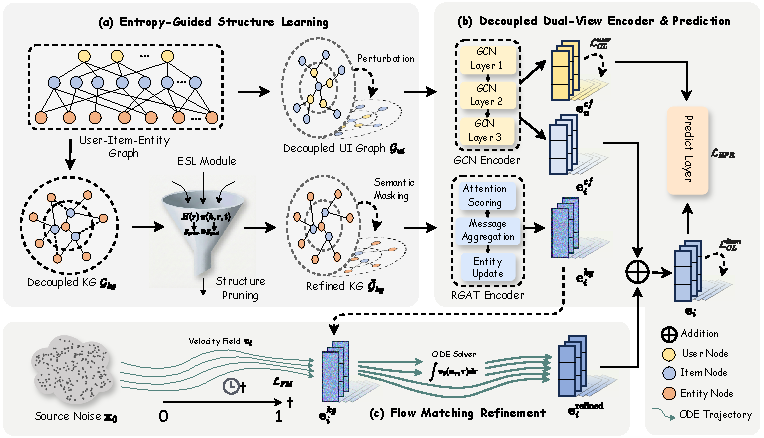
\includegraphics[width=\textwidth]{image/model2.pdf}
	\caption{Schematic overview of the proposed FlowKG framework. It incorporates an entropy-guided module for pre-filtering KG structure, a decoupled encoder for dual-view representation learning, and a flow matching module to refine latent embeddings via optimal transport paths.}
	\label{fig:model}
\end{figure*}


\subsection{Problem Formulation}
We model the task as link prediction within a heterogeneous information network.

\subsubsection{\textbf{User-Item Interaction Graph}}
Let $\mathcal{U}$ and $\mathcal{I}$ denote the sets of users and items, respectively. The historical interactions between users and items are represented as a bipartite graph $\mathcal{G}_{ui} = (\mathcal{U} \cup \mathcal{I}, \mathcal{E}_{ui})$, where each edge $(u, i) \in \mathcal{E}_{ui}$ indicates an observed interaction between user $u$ and item $i$.

\subsubsection{\textbf{Knowledge Graph (KG)}}
To incorporate auxiliary semantic information, we utilize a Knowledge Graph $\mathcal{G}_{kg} = (\mathcal{E}, \mathcal{R}, \mathcal{T})$, where $\mathcal{E}$, $\mathcal{R}$, and $\mathcal{T}$ represent the sets of entities, relations, and triplets, respectively. Items are mapped to corresponding entities within this graph, i.e., $\mathcal{I} \subseteq \mathcal{E}$. This mapping enriches the representation of items with contextual information, such as relations like (Movie, Director, Person).

\subsubsection{\textbf{Task Definition}}
Given $\mathcal{G}_{ui}$ and $\mathcal{G}_{kg}$, the objective is to learn a scoring function $\hat{y}_{ui} = f_\Theta(u, i)$ that predicts the likelihood of user $u$ interacting with an unobserved item $i$, generating a Top-$K$ ranking list. The goal is to generate a ranked list of Top-$K$ recommendations for each user.

\subsection{Flow Matching with Optimal Transport}
Flow Matching (FM) is a generative modeling framework grounded in the theory of Continuous Normalizing Flows (CNFs)~\cite{chen2018neural,grathwohl2018ffjord}. In contrast to diffusion models that rely on stochastic differential equations (SDEs)~\cite{ho2020denoising,song2020score}, FM constructs a deterministic probability path that transforms samples from a simple prior distribution $p_0$ (e.g., a Gaussian) into samples from the complex target data distribution $q(\mathbf{x})$.
The generative process is governed by an ordinary differential equation (ODE):
\begin{equation}
	\frac{\mathrm{d}\mathbf{x}_t}{\mathrm{d}t} = \mathbf{v}_t(\mathbf{x}_t; \theta), \quad t \in [0, 1],
\end{equation}
where $\mathbf{v}_t$ is a time-dependent vector field parameterized by a neural network. By numerically integrating this ODE, one can map an initial noise sample $\mathbf{x}_0 \sim p_0$ to a generated data sample $\mathbf{x}_1 \sim q(\mathbf{x})$.

To enable stable and efficient training, we adopt Conditional Flow Matching with Optimal Transport (OT) paths~\cite{tong2024improving}. An OT path corresponds to the straight-line interpolation between a source noise sample $\mathbf{x}_0$ and a target data sample $\mathbf{x}_1$, which minimizes the transport cost:
\begin{equation}
	\psi_t(\mathbf{x}_0, \mathbf{x}_1) = (1 - t)\mathbf{x}_0 + t \mathbf{x}_1.
\end{equation}
Differentiating this path with respect to time yields a simple, time-independent conditional vector field $\mathbf{u}_t$:
\begin{equation}
	\mathbf{u}_t(\mathbf{x} | \mathbf{x}_1) = \mathbf{x}_1 - \mathbf{x}_0.
\end{equation}
This implies that the learned model $\mathbf{v}t$ only needs to regress the constant displacement vector pointing from the noise to the target data sample. Consequently, the training objective simplifies to regressing this conditional vector field:
\begin{equation}
	\mathcal{L}_{\text{fm}}(\theta) = \mathbb{E}_{t, \mathbf{x}_0, \mathbf{x}_1} \left[ \| \mathbf{v}_t(\psi_t(\mathbf{x}_0, \mathbf{x}_1); \theta) - (\mathbf{x}_1 - \mathbf{x}_0) \|^2 \right].
	\label{eq:fm_loss}
\end{equation}
This straightforward and efficient formulation provides the mathematical basis for the representation refinement module in our framework.

%\subsection{\textbf{Problem Formulation}}
%We formulate the KG-enhanced recommendation task as a link prediction and ranking problem within a heterogeneous information network.
%
%\subsubsection{\textbf{User-Item Interaction Graph}}
%Let $\mathcal{U} = \{u_1, u_2, \dots, u_M\}$ denote the set of users and $\mathcal{I} = \{i_1, i_2, \dots, i_N\}$ denote the set of items, where $M$ and $N$ represent the number of users and items, respectively. The historical interaction data is constructed as a bipartite graph $\mathcal{G}_{ui} = (\mathcal{U} \cup \mathcal{I}, \mathcal{E}_{ui})$, where the edge set $\mathcal{E}_{ui}$ contains all observed interaction pairs $(u, i)$ (indicating implicit feedback $y_{ui}=1$).
%
%\subsubsection{\textbf{Knowledge Graph (KG)}}
%To incorporate external semantic information, we utilize a Knowledge Graph $\mathcal{G}_{kg} = (\mathcal{E}, \mathcal{R}, \mathcal{T})$. Here, $\mathcal{E}$ represents the set of entities, $\mathcal{R}$ is the set of relations, and $\mathcal{T} = \{(h, r, t) | h, t \in \mathcal{E}, r \in \mathcal{R}\}$ denotes the collection of triplets. In the recommendation scenario, the item set typically maps to a subset of the entity set, i.e., $\mathcal{I} \subseteq \mathcal{E}$. The KG provides rich semantic contexts for items (e.g., ``Movie-Director'' or ``Product-Brand'' associations).
%
%\subsubsection{\textbf{Task Definition}}
%Given the interaction graph $\mathcal{G}_{ui}$ and the knowledge graph $\mathcal{G}_{kg}$, our goal is to learn a scoring function $\hat{y}_{ui} = f_\Theta(u, i)$ to predict the preference probability of user $u$ for an unobserved item $i$. Based on these predicted scores, the system generates a Top-$K$ recommendation list sorted in descending order of preference for each user.
%
%\subsection{Flow Matching for Generative Modeling}
%Flow Matching (FM)~\cite{lipman2022flow} is a generative paradigm based on Continuous Normalizing Flows (CNF), designed to achieve distribution mapping by regressing a vector field along a fixed probability path. Compared to diffusion models, FM avoids complex Stochastic Differential Equation (SDE) simulations, offering more deterministic generation trajectories and more stable training objectives.
%
%\subsubsection{\textbf{Continuous Normalizing Flows via ODE}}
%FM models the sample generation process as a time-dependent probability density path $p_t(x)$ where $t \in [0, 1]$. This process is described by an Ordinary Differential Equation (ODE):
%\begin{equation}
%	\frac{\mathrm{d}x_t}{\mathrm{d}t} = v_t(x_t; \theta), \quad x_0 \sim p_0(x),
%\end{equation}
%where $x_t \in \mathbb{R}^d$ is the state vector, $v_t$ is the velocity vector field parameterized by a neural network, and $p_0$ is a known prior distribution (typically set as the standard Gaussian distribution $\mathcal{N}(0, \mathbf{I})$). By numerically integrating this ODE from $t=0$ to $t=1$, noise samples $x_0$ can be mapped to data samples $x_1$ that follow the target data distribution $p_1(x) \approx q(x)$.
%
%\subsubsection{\textbf{Conditional Flow Matching with Optimal Transport}}
%In practice, directly regressing the vector field of the marginal probability path is often intractable. Conditional Flow Matching (CFM) addresses this by introducing a conditional variable (i.e., the target data point $x_1$) to marginalize the vector field, thereby enabling efficient training without simulating ODE trajectories.
%
%Within the CFM framework, the **Optimal Transport (OT)** path has garnered significant attention due to its straight generation trajectories and minimal transport cost. The OT path is typically defined as a linear interpolation between the source noise $x_0$ and the target data $x_1$:
%\begin{equation}
%	\psi_t(x_0, x_1) = (1 - t)x_0 + t x_1.
%\end{equation}
%Differentiating this path with respect to time $t$ yields a constant closed-form solution for its corresponding conditional vector field:
%\begin{equation}
%	u_t(x | x_1) = x_1 - x_0.
%\end{equation}
%This concise form implies that the neural network $v_t$ only needs to learn to predict the ``displacement direction'' pointing from noise to data. Consequently, the training objective of FM simplifies to regressing this conditional vector field, with the loss function defined as:
%\begin{equation}
%	\mathcal{L}_{FM}(\theta) = \mathbb{E}_{t \sim \mathcal{U}[0,1], x_0 \sim p_0, x_1 \sim q(x)} \left[ \| v_t(\psi_t(x_0, x_1); \theta) - (x_1 - x_0) \|^2 \right].
%	\label{eq:fm_loss}
%\end{equation}
%During the inference phase, given an initial noise $x_0$, the model reconstructs the data representation by advancing along the learned vector field using a numerical solver (e.g., the Euler method).